\chapter{Introduction}

Fluid flows are an important part of everyday life. Fluid mechanics is a whole discipline dedicated
to studying and describing the behaviour of liquids and gasses in motion. More and more industrial
and scientific applications surface everyday, from great scales like climate studies encompassing
the whole earth over millennia, to the study of microscopic cells flowing through tiny blood
vessels. The aerospace industry is probably the most evident example of how prevalent aerodynamics
are in today's world. Before the advent of computers, there were really only two methods used in
engineering fluid dynamics: experimental and theoretical. Since the widespread use of computers
became the norm, a third method appeared: \textit{\acrfull{acr:CFD}}. This is a numerical approach
to solving the equations governing those processes.

Usage of \acrshort{acr:CFD} has been steadily rising in recent years~\cite{Slotnick2014}. It is easy
to imagine why, when experimental results are so costly to obtain, and a theoretical approach is
difficult to apply to complex cases. Nonetheless, \acrshort{acr:CFD} is not meant to replace those
methods, but to be combined with them: reducing the need to perform experiments, while comparing
results with those from actual experiments to verify and validate the numerical
models~\cite{Stern2001}.

Even with increasing computing power, some problems are difficult to solve with \acrshort{acr:CFD}.
Problems of high-dimensionality and complex flows still cannot be solved economically. NASA's
\acrshort{acr:CFD} Vision 2030 study~\cite{Slotnick2014} states that turbulent flow separation is
one area that still cannot be predicted accurately. In order to simulate these problems, we will
need increased processing power, more efficient use of that power, and higher resolution numerical
methods.

% DG-SEM
Spectral methods are an answer to that need of more accurate numerical methods. Unlike traditional
methods like finite differences methods, finite element methods and finite volume methods, spectral
methods are high-order methods and converge exponentially fast. Such methods are used to solve
complex flows, but are expensive and are only recently emerging from the research environment to
tackle more and more complex problems from classical aerodynamics~\cite{Vadsola2021} to nuclear
reactor flows~\cite{Merzari2017}, internal combustion~\cite{Wu2021}, ocean
simulation~\cite{Molcard2002}, atmosphere simulation~\cite{Haidvogel1997}, and more. 

\begin{figure}[H]
	\centering
	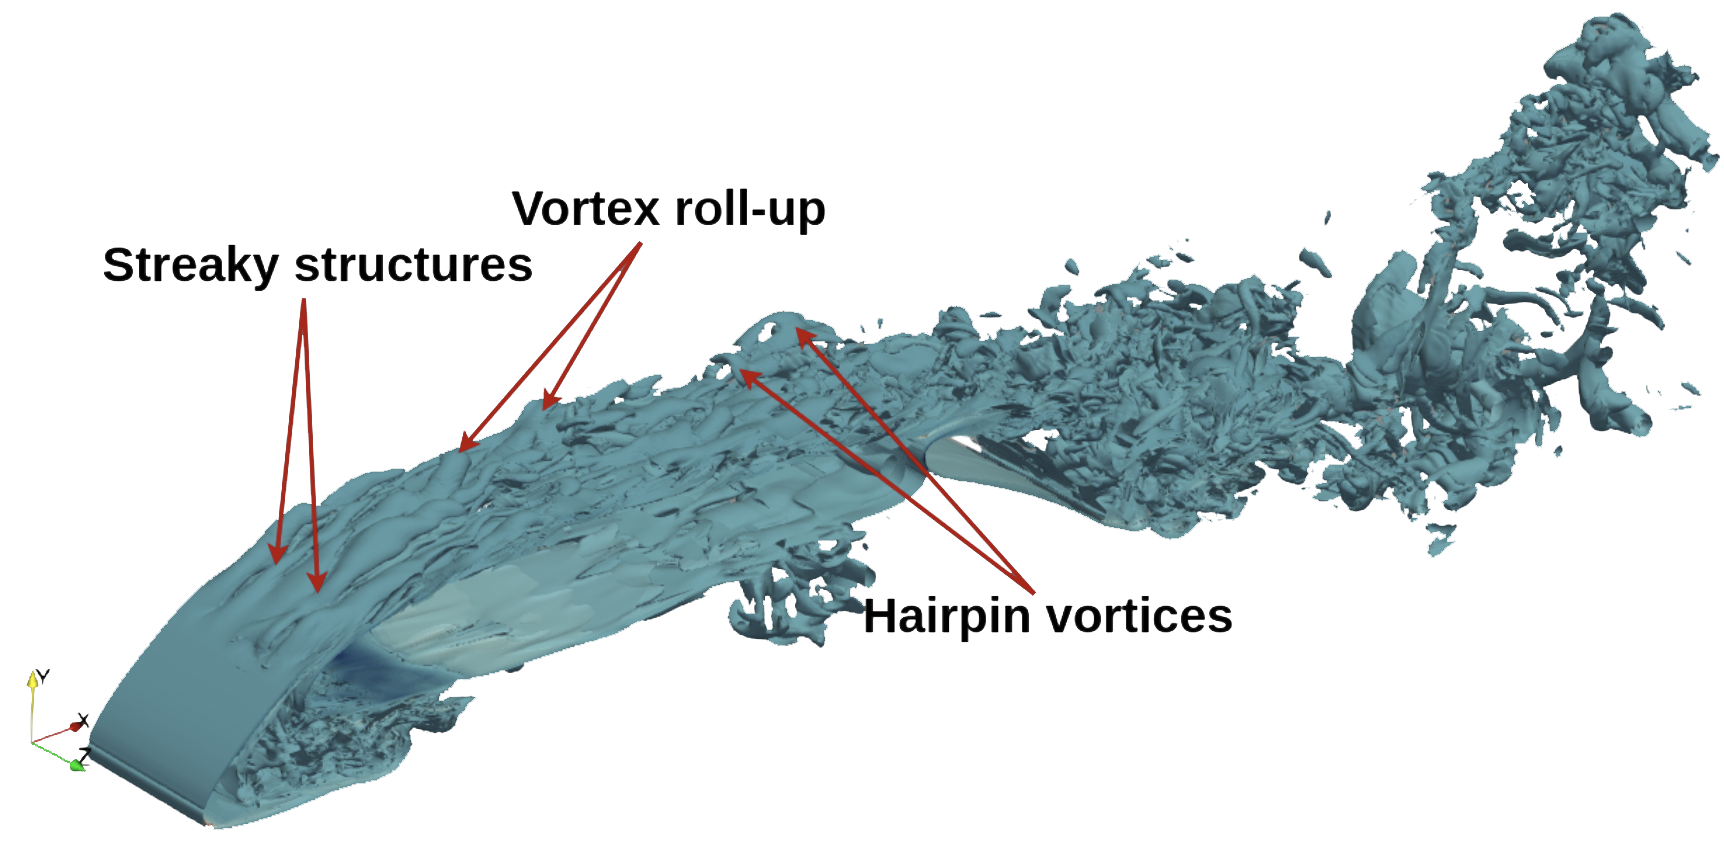
\includegraphics[width=0.95\textwidth]{Chapter_introduction/media/spectral_element_method}
	\caption{Direct numerical simulation: Spectral methods have sufficient accuracy to model very complex flows (reprinted from~\cite{Vadsola2021}).}\label{fig:intro_sem}
\end{figure}

Instead of modelling the solution as individual values at points, or a linear or quadratic function
within a space subdivision, spectral methods represent a function as a truncated series:

\begin{equation}
	u(x) \approx u_N(x) = \sum_{n = 0}^{N} \widehat{u}_n \phi _n(x),
\end{equation}

\noindent
where \(\phi _n(x)\) are basis functions. We use this representation in the governing equations to
compute the unknowns \(\widehat{u}_n\). Spectral methods are usually divided into two
categories~\cite{Karniadakis2005}: collocation methods and Galerkin methods. Galerkin methods solve
governing equations in integral form over the domain~\cite{Reed1973}, which is broken up into
elements. This method, in combination with the spectral approximation, will be used in this work. It
is called the \textit{Galerkin spectral element method}. This method can be formulated both in
\textit{continuous} and \textit{discontinuous} versions. Continuous methods decompose the domain
into elements, within which the solution is represented as functions. These functions join at the
element boundaries, making the method continuous. Discontinuous methods allow the solution to be
discontinuous at element boundaries, using fluxes between elements to stabilise the scheme. We refer
to these as the \textit{\acrfull{acr:DG-SEM}}. We will use this method, as it is easier to be made
parallel. The fact that elements are independent and only connect through fluxes should map better
to the \acrshort{acr:GPU} architecture, where the solution of all elements will be computed
concurrently. It also simplifies mesh refinement by simplifying the usage of non-conforming
interfaces. Both \acrshort{acr:SEM} methods, continuous or discontinuous, combines the accuracy and
exponential convergence of spectral methods with the geometric flexibility of finite element
methods. 

% GPUs
With the stagnation of traditional computer \textit{\acrfull{acr:CPU}} operating frequencies over
the last years~\cite{Parkhurst2006}, computer systems have evolved to use more parallel
architectures. \Acrshortpl{acr:CPU} are now composed of several computing cores~\cite{Nayfeh1997}
executing tasks together or in parallel, and contemporary \textit{\acrfull{acr:HPC}} platforms
consist of several whole computers networked together executing tasks in parallel. Amidst those
changes, an inherently parallel architecture has started to be used in scientific computing.
\textit{\Acrfullpl{acr:GPU}} are computer chips that were initially used in computer graphics, for
massively parallel workloads. \Acrshortpl{acr:GPU} can now be programmed similarly to traditional
\acrshortpl{acr:CPU}~\cite{Owens2008}, offering their thousands of simpler cores to many kinds of
computation. This architecture is optimised for maximal bandwidth, to process great amounts of data
as fast as possible. Recently, these processors have been incorporated into \acrshort{acr:HPC}
platforms~\cite{Fan2004}, enabling massively parallel workloads with theoretical processing power
much greater than that using traditional \acrshortpl{acr:CPU}.

\begin{figure}[H]
	\centering
	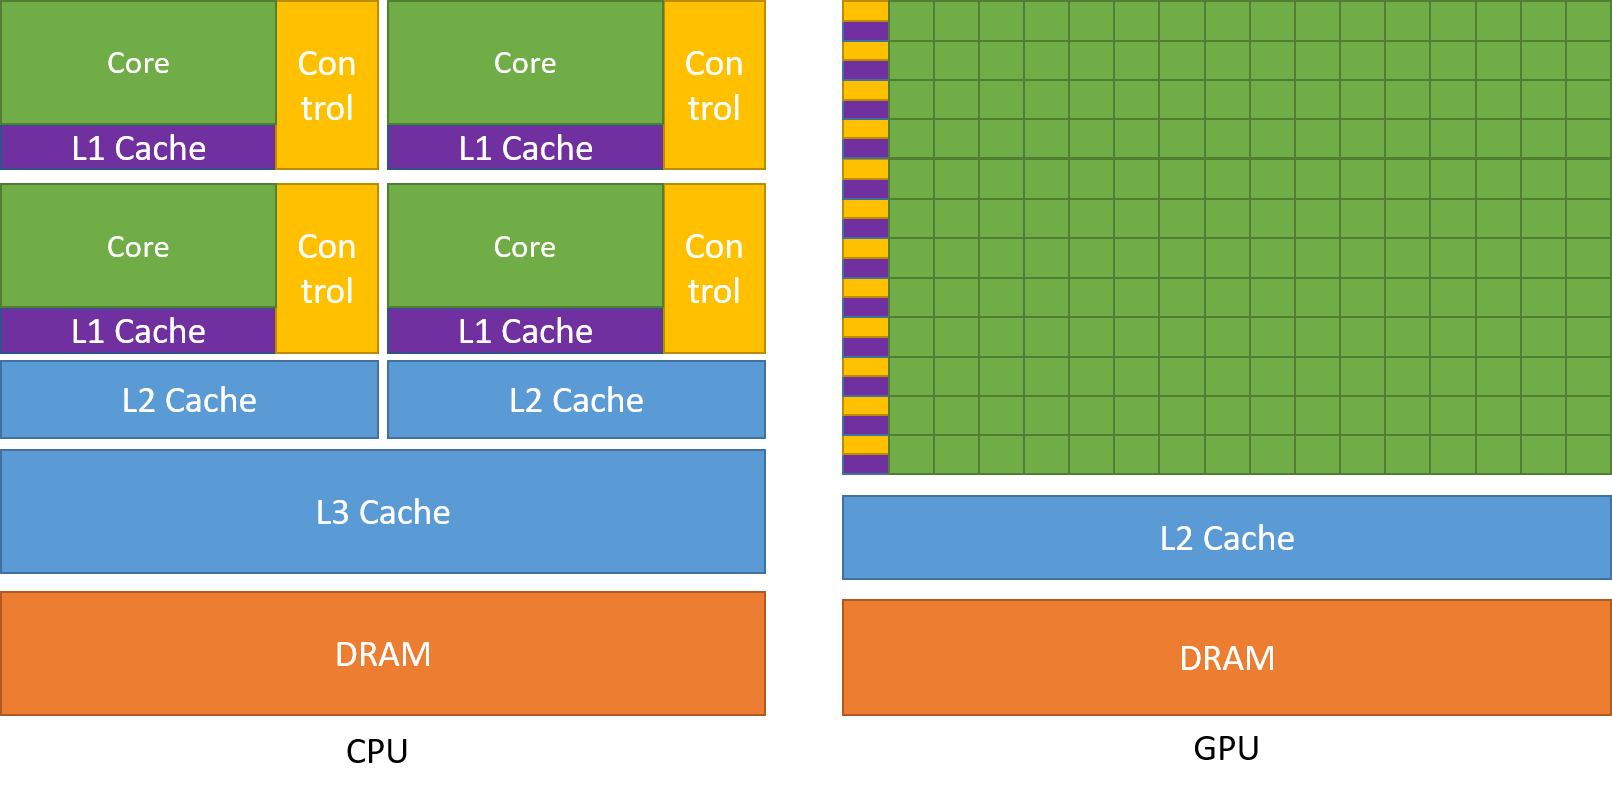
\includegraphics[width=0.8\textwidth]{Chapter_introduction/media/gpu-devotes-more-transistors-to-data-processing}
	\caption{\Acrshort{acr:GPU} architecture~\cite{Nvidia2021}: \Acrshortpl{acr:GPU} dedicate much more die space to computations (in green).}\label{fig:intro_gpu}
\end{figure}

We will use \acrshortpl{acr:GPU} for our computations in the hope of increasing the available
processing power to solve complex problems. This will not come easily, as \acrshort{acr:GPU}
architectures are optimised for static workloads executing the exact same code on all
\acrshort{acr:GPU} cores. We use the \acrshort{acr:CUDA} parallel computing
platform~\cite{Garland2008}, which enables programming \acrshortpl{acr:GPU} using the C++ language
with some extensions, much like \acrshort{acr:CPU} programming.

% Adaptivity
Even with highly accurate methods and the processing power of \acrshort{acr:GPU}-enabled
\acrshort{acr:HPC} platforms, the available resources must be spent judiciously. To get the accurate
results we want, meshes need to be extremely fine. A mesh this fine throughout the whole domain can
become impractical to compute even on the largest \acrshort{acr:HPC} systems. The limited resources
must be spent where they will count most. Creating grids that are more refined in areas of interest
is possible if those areas are known beforehand. This is a time-consuming process that must be
started over for every new problem. It is sometimes not possible to predict where areas of interest
will be, such as when modeling chaotic turbulent flows. It is also possible that the mathematically
important areas are not easy to identify. 

\textit{\Acrfull{acr:AMR}} methods have been developed in order to solve this problem. These methods
aim to identify the areas of the mesh that need refinement, and refine those areas to obtain more
accurate results while not wasting resources on areas of less interest. Figure~\ref{fig:intro_amr}
shows a problem that has been refined in order to better capture the bow shock around a spacecraft.
In 1984, Berger and Oliger~\cite{Berger1984} described a recursive method where refined grids can
contain further refined grids, used for the finite difference method and hyperbolic equations.
Another \acrshort{acr:AMR} method by Khokhlov~\cite{Khokhlov1998} has reported a factor of 10
savings of both memory and computing time. We will use \acrlong{acr:AMR} to make more efficient use
of the resources we have and to ease working with the more limited amount of memory of
\acrshortpl{acr:GPU} compared to \acrshortpl{acr:CPU}.

\begin{figure}[H]
	\centering
	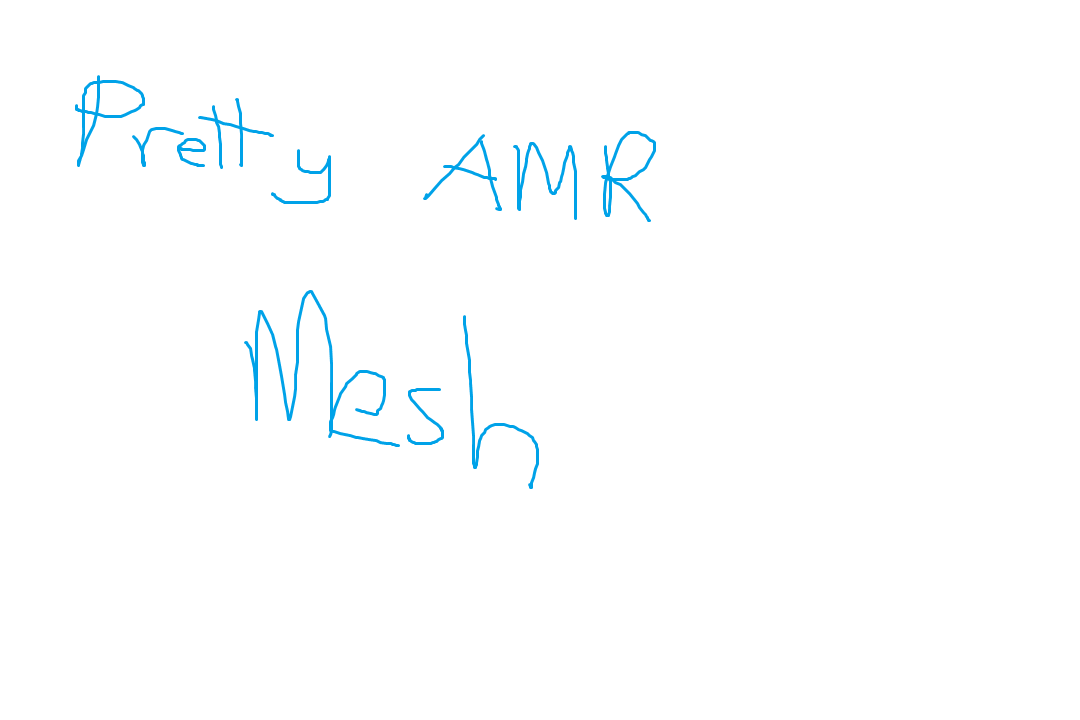
\includegraphics[width=0.8\textwidth]{Chapter_introduction/media/adaptive_mesh_refinement}
	\caption{\Acrlong{acr:AMR}: The mesh is more refined in certain flow regions to capture important features of the flow (reprinted from~\cite{Siemens2020}).}\label{fig:intro_amr}
\end{figure}

Two general approaches to \acrshort{acr:AMR} exist. Berger and Oliger~\cite{Berger1984} use
\textit{block-structured} \acrshort{acr:AMR}, where uniformly refined meshes are overlaid on coarse
meshes, as shown in Figure~\ref{fig:block_structured}. Another approach is \textit{tree-structured}
\acrshort{acr:AMR}, where elements themselves are refined recursively as in
Figure~\ref{fig:tree_structured}. Khokhlov~\cite{Khokhlov1998} describes such an approach that works
fully in parallel. We will use a tree-structured approach, since it can easily work in parallel by
having elements refine independently.

\begin{figure}[H]
	\centering
	\subfloat[Block-structured \acrlong{acr:AMR}]
	{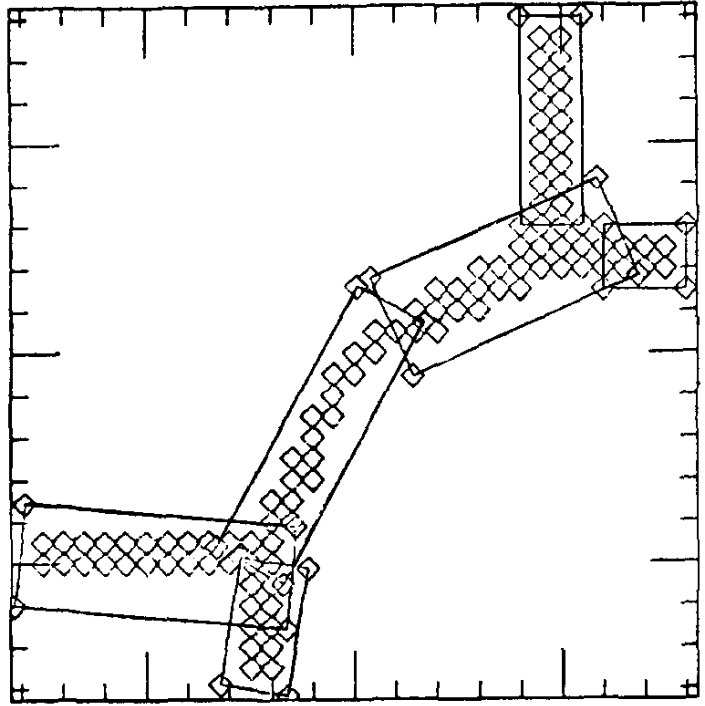
\includegraphics[width=0.45\textwidth]{Chapter_introduction/media/block_structured}\label{fig:block_structured}}
	\hfill
	\subfloat[Tree-structured \acrlong{acr:AMR}]
	{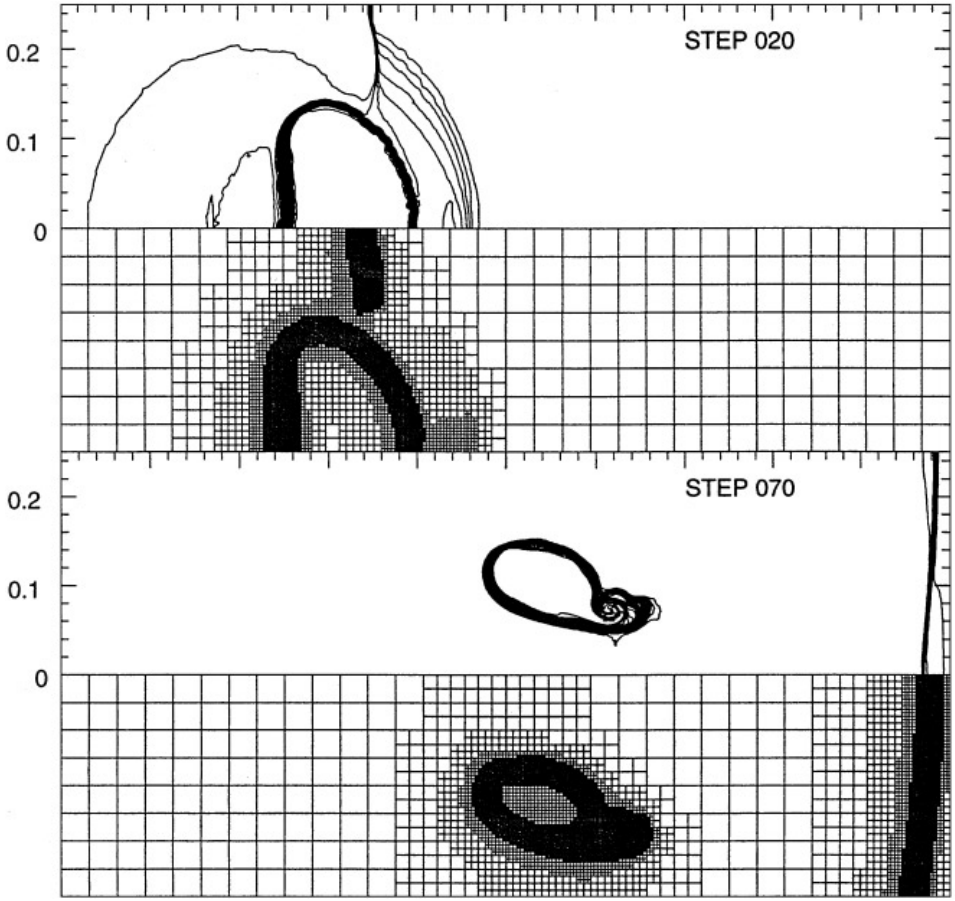
\includegraphics[width=0.45\textwidth]{Chapter_introduction/media/tree_structured}\label{fig:tree_structured}}
	\caption{\Acrlong{acr:AMR} approaches: Two different approaches to refining the important areas of a mesh. (a) Finer meshes are patched onto the initial coarse mesh (reprinted from~\cite{Berger1984}) (b) Elements are refined individually (reprinted from~\cite{Khokhlov1998})}\label{fig:amr_structures}
\end{figure}

Two types of refinement will be used in this work. \textit{p-refinement} increases the polynomial
order of the spectral approximation inside an element, increasing the number of collocation points
inside the element. \textit{h-refinement} splits elements into smaller elements, increasing the
number of elements in the mesh.

The choice of which refinement type to use, as well as the choice of which area of the mesh to
refine is guided by an error estimator. Mavriplis~\cite{Mavriplis1990} describes an \textit{a
posteriori error estimator} that uses the spectral approximation to estimate the error and the
smoothness of the solution. The smoothness of the solution is used to determine which refinement
type is expected to increase accuracy the most. Elements with a high error get refined, using
p-refinement if their solution is smooth or h-refinement if it is not.

The benefits of \acrshort{acr:AMR} do not come without added complications. Two main complications
are: non-conforming interfaces and load imbalance.

% Mortar element method
As the mesh refines, it becomes non-uniform. Elements can have neighbours with a different
polynomial order, different sizes, or both. The interfaces between such elements are called
\textit{non-conforming interfaces}. Such interfaces can be \textit{functionally non-conforming},
\textit{geometrically non-conforming}, or both. Figure~\ref{fig:intro_interfaces} shows these
different types of interfaces. Several methods have been developed to deal with these interfaces. We
use the \textit{mortar element method}~\cite{Maday1989}, as it retains the exponential convergence
of spectral methods.

\begin{figure}[H]
	\centering
	\subfloat[Conforming interface]
	{\includesvg[width=0.45\textwidth]{Chapter_introduction/media/conforming_interface_N4}\label{fig:intro_conforming_interface}}
	\hfill
	\subfloat[Non-conforming interfaces]
	{\includesvg[width=0.45\textwidth]{Chapter_introduction/media/non_conforming_interfaces_N4_N6}\label{fig:intro_non_conforming_interfaces}}
	\caption{Two types of interfaces: Interfaces can be either conforming or non-conforming. (a) The collocation points line up (b) The collocation points do not line up}\label{fig:intro_interfaces}
\end{figure}

% Load balancing
The second complication of \acrshort{acr:AMR} is load imbalance. Solving the problem on multiple
\acrshortpl{acr:GPU} splits the mesh into blocks, one per \acrshort{acr:GPU}. As the mesh is
refined, it is unlikely that all blocks are refined equally. Every \acrshort{acr:GPU} must
synchronise at every time step, therefore \acrshortpl{acr:GPU} with less work to execute will be
waiting while the more heavily loaded \acrshortpl{acr:GPU} finish their computations. The simulation
time will be driven by the most heavily loaded \acrshort{acr:GPU}, which will degrade performance on
parallel systems. Figure~\ref{fig:intro_load_balancing} shows an imbalanced system.


\begin{figure}[H]
	\centering
	\subfloat[Mesh before refining]
	{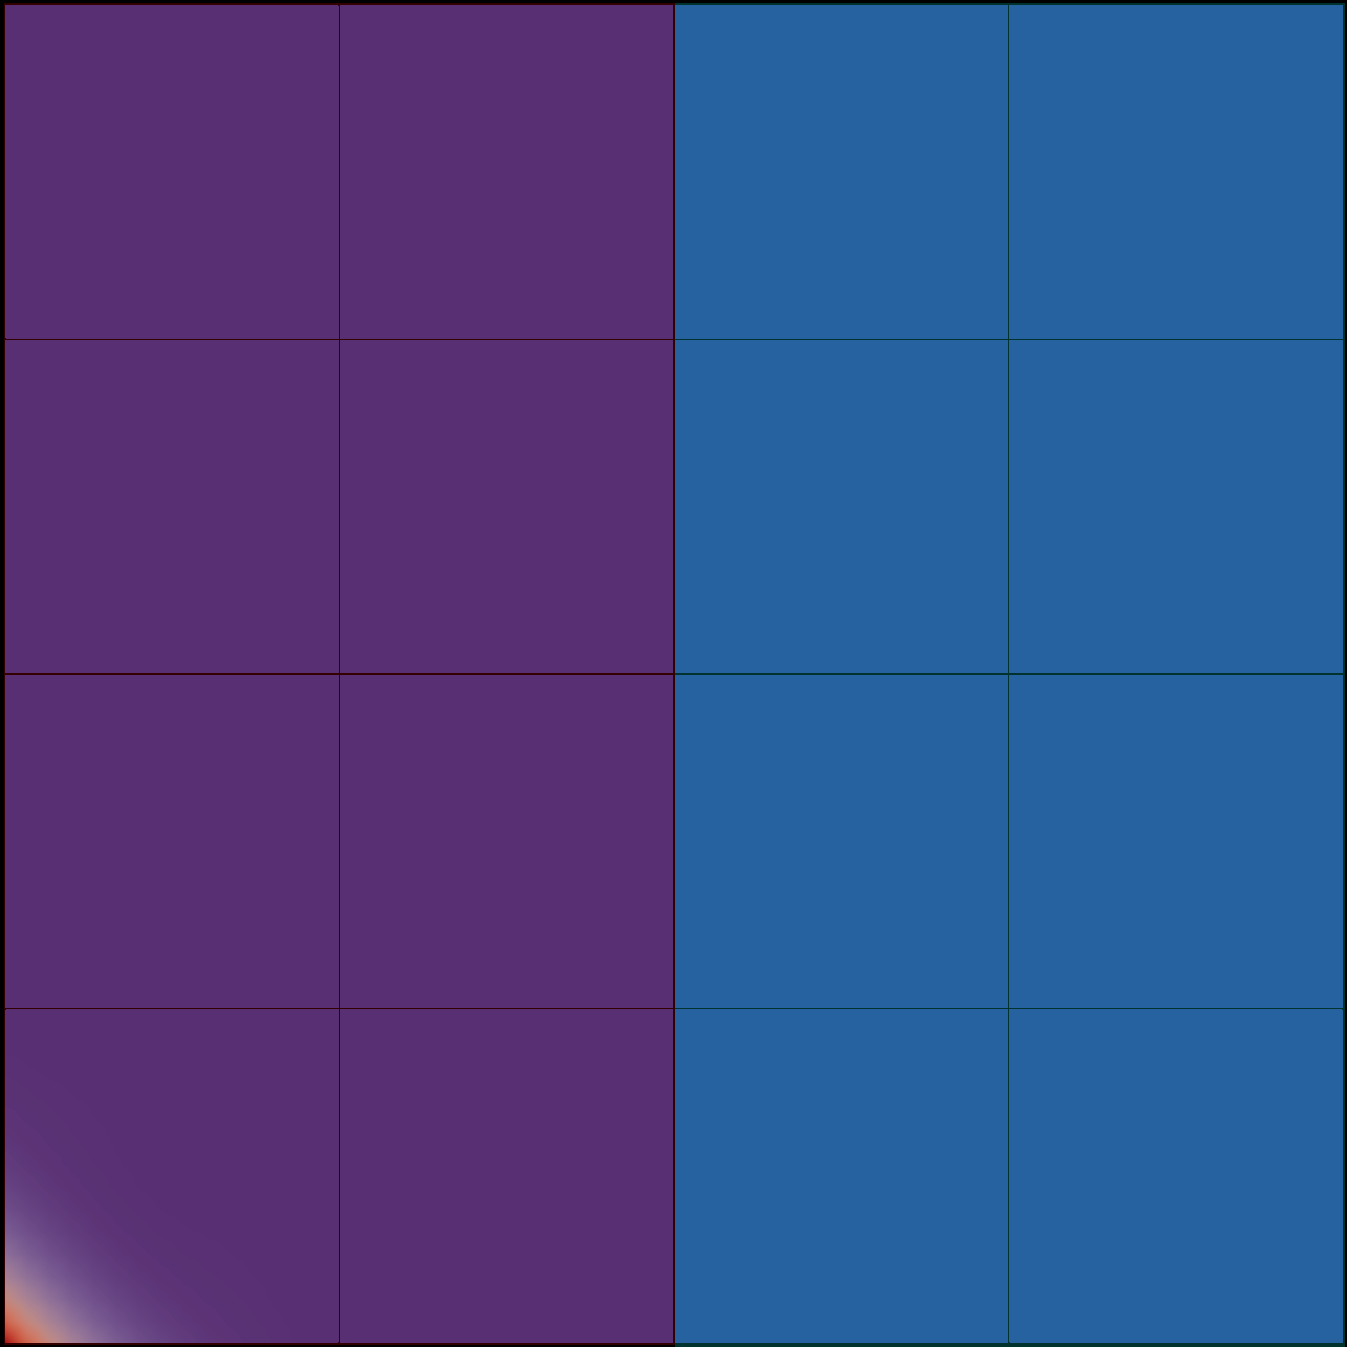
\includegraphics[width=0.45\textwidth]{Chapter_introduction/media/load_imbalance_initial}\label{fig:intro_mesh_imbalance_initial}}
	\hfill
	\subfloat[Mesh after refining]
	{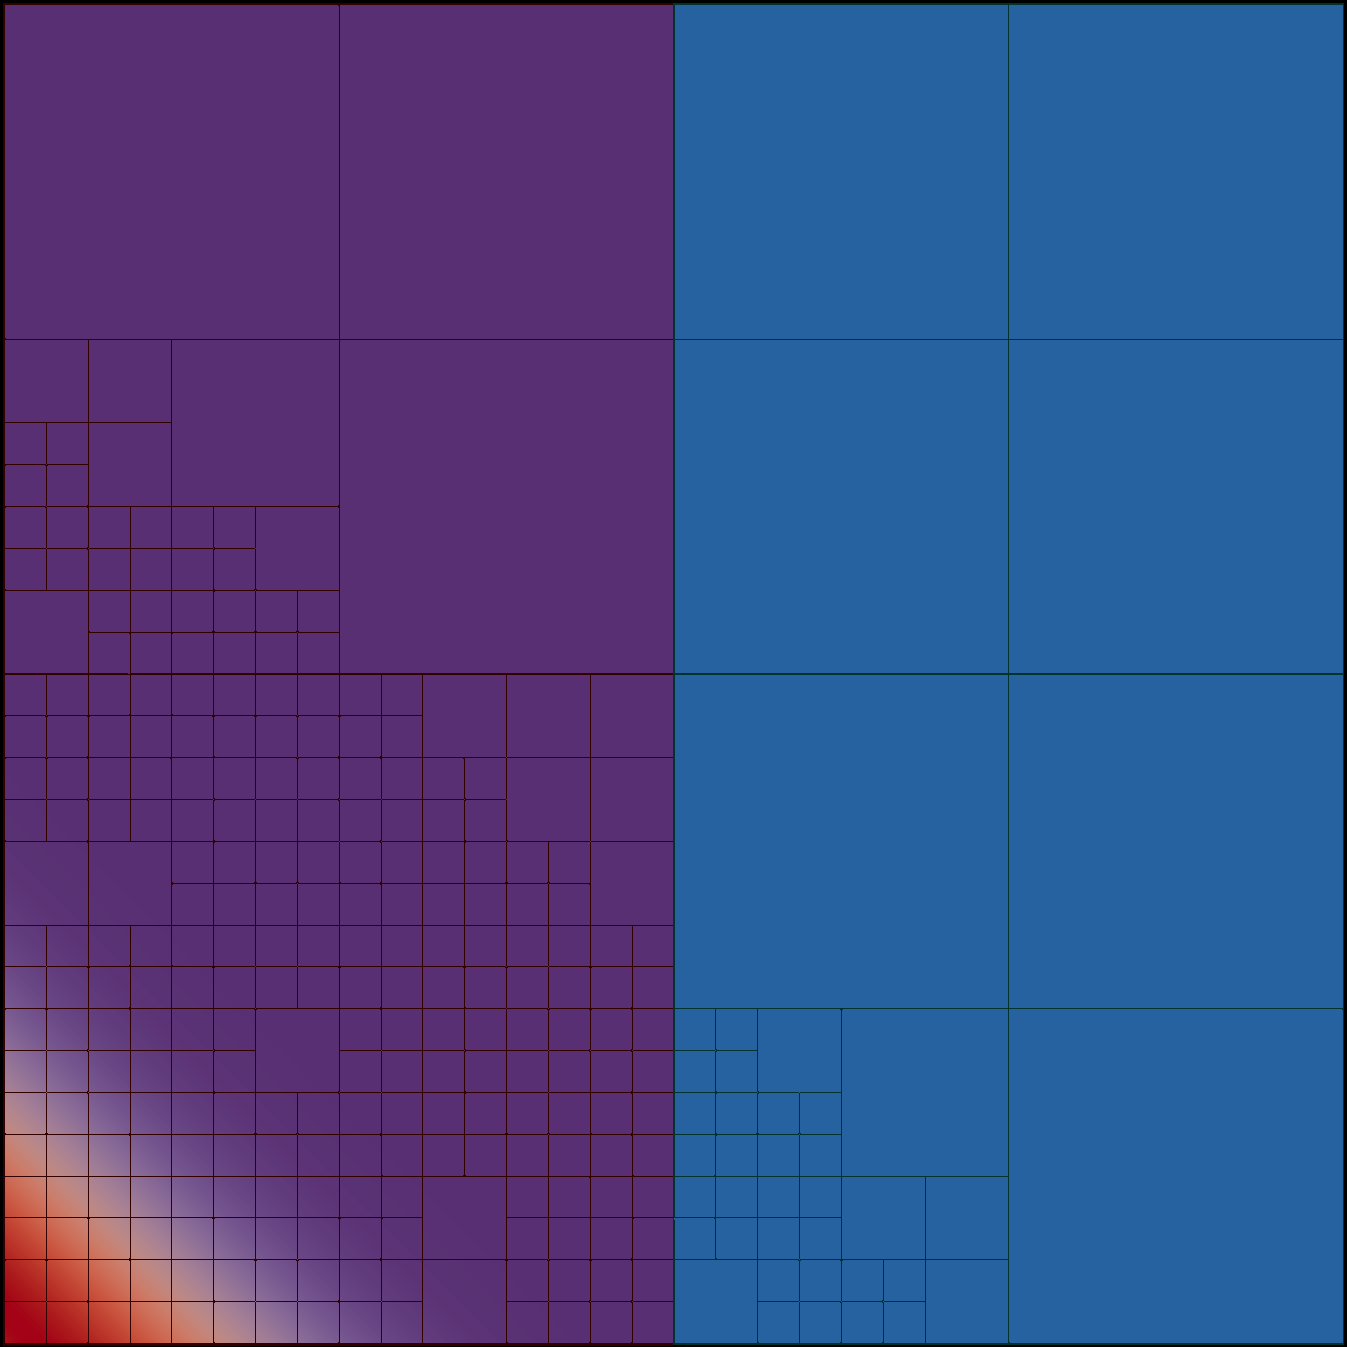
\includegraphics[width=0.45\textwidth]{Chapter_introduction/media/load_imbalance}\label{fig:intro_mesh_imbalance_after_refinement}}
	\caption{Load imbalance: The elements have split unequally in the two worker \acrshortpl{acr:GPU}, purple and blue, one having a higher computational load. (a) Before refining (b) After refining}\label{fig:intro_load_balancing}
\end{figure}

In order to avoid this problem, the mesh needs to be repartitioned as it is refined. This is the
process of \textit{dynamic load balancing}. When the mesh is repartitioned, elements are sent
between \acrshortpl{acr:GPU} to even out their computational load. The repartitioning scheme
dictates which elements are sent from one \acrshort{acr:GPU} to another. This scheme should satisfy
several conditions: it must even the load between the workers, it must be fast to execute, and it
must minimise the boundaries between the mesh blocks it creates. 

Many approaches to this problem have been studied. \textit{Graph-based} repartitioning schemes
represent a mesh as nodes connected by edges, which can then be partitioned by splitting it into
parts of equal size while severing as few edges as possible. The well-known
\textit{Metis}\cite{Karypis1998} library uses this technique. Graph-based techniques produce very
well partitioned meshes, but can be slower to execute than other techniques and need to know the
topology of the entire mesh to partition it, which can be a problem on parallel systems where the
problem should be split between the different workers.

A different approach is \acrfull{acr:SFC} based repartitioning schemes. These schemes reduce
multidimensional problems to one dimension by mapping elements to a single curve going through the
entire domain\cite{Peano1890}. The elements can then be indexed in 1D, and repartitioned by
splitting that line into segments of equal size. \Acrshortpl{acr:SFC} are very fast to generate,
which is especially relevant to this work as the repartitioning will be performed often while the
computation is underway. Some curves, like the \textit{Hilbert curve}~\cite{Hilbert1891}, retain a
very good locality, which will help reduce the size of inter-block boundaries. This can improve the
performance of the program by reducing the amount of communication between \acrshortpl{acr:GPU}. In
this work, we will implement a \acrshort{acr:SFC} based repartitioning scheme using the Hilbert
curve in order to perform dynamic load balancing.

% Problem
In summary, we want to solve complex problems with high accuracy. We will need a high resolution
numerical method, more processing power than traditional \acrshort{acr:CPU} programming methods
possess, and a way to use that increased processing power as efficiently as possible. 

We propose using the \acrlong{acr:DG-SEM} as a very accurate numerical method. We will perform the
computations on \acrlongpl{acr:GPU} to access their great amount of parallel processing power. We
will use this increased amount of computing power more efficiently by performing \acrlong{acr:AMR}
to use more ressources where needed, and less elsewhere. We will finally add dynamic load balancing
to keep the parallel efficiency of the program as high as possible while the topology changes. This
tackles the main challenges necessary to keep advancing \acrshort{acr:CFD}.

In order to showcase these techniques, we will solve a sample problem using the 2D wave equation:

\begin{gather}
	\frac{\partial^2p}{\partial t^2} - c^2(p_{xx} + p_{yy}) = 0 \\
	u_t = - p_x \\
	v_t = -p_y.
\end{gather}

% Structure
The structure of this thesis will follow these main concepts.
Chapter~\ref{chapter:literature_review} discusses the current state of the art of the domain.
Chapter~\ref{chapter:graphics_processing_units} presents the \acrshort{acr:GPU} architecture and how
we tackle implementing our algorithms to that special architecture. In
Chapter~\ref{chapter:spectral_element_method}, we present the \acrshort{acr:DG-SEM} and the
derivation used for the sample problem. Then, Chapter~\ref{chapter:adaptive_mesh_refinement}
explains our proposed algorithm for parallel \acrshort{acr:AMR} on \acrshortpl{acr:GPU}. We then
present a solution to perform dynamic load balancing and the challenges of a dynamic mesh structure
in Chapter~\ref{chapter:load_balancing}. The performance of the program, as well as several
comparisons of the impact of the different features using \acrshort{acr:HPC} systems are presented
in Chapter~\ref{chapter:results}. We conclude with Chapter~\ref{chapter:conclusion}, and present
ideas for future work.
